
\section{The circular system $\CTlambda$}
We introduce  a condition call \emph{global trace condition} for all proofs $\Pi$ that the term $t$ is well-typed,
then the subset $\GTC$ of the set $\WTyped$ of well-typed terms of $\LAMBDA$ 
satisfying the global trace condition. $\GTC$ is a set of total recursive functionals. We use $\GTC$
as a semantics for the set $\CTlambda$ of circular $\lambda$-terms we will define.

$\CTlambda$ will be the regular terms of $\CTlambda$. 
$\CTlambda$ is a decidable set.
For the terms of $\CTlambda$ we will prove
strong normalization, church-rosser for the \quotationMarks{safe} part of a term, 
and the fact that every closed normal term of type
$\N$ is a numeral. 
As a consequence, all terms $\CTlambda$ will be interpreted as total functionals. 
\\

From the $\N$-argument connection we now define the global trace condition and the set of 
terms of $\GTC$  and of $\CTlambda$.



\begin{definition}[Global trace condition and terms of $\CTlambda$]
\label{definition-global-trace-condition}
\mbox{}
 \linebreak 
Assume $\tau =( (k_m,t_m), \ldots, (k_n,t_n), \ldots)$ 
is a trace of a path $\pi = (t_1, \ldots, t_n, \ldots)$ of $t \in \WTyped$. 
Assume $i=m,\ldots, n$.
\begin{enumerate}
\item
$\tau$ is progressing in $i$ if $t_i=\cond(f,g)$ for some $f$, $g$,
and $k_i$ is the index of the first \emph{unnamed} argument the $\cond$-rule, 
otherwise $\tau$ is not progressing in $i$.

\item
$t$ satisfies the global trace condition if for some typing proof $\Pi$,
of $t$, for all infinite paths $\pi$ of $t$ in $\Pi$,
there is some infinitely progressing path $\tau$ in $\pi$ and $\Pi$.
$\GTC$ is the set of well-typed terms $t \in \LAMBDA$ satisfying the global trace condition.

\item
$\CTlambda = \GTC \cap \Reg$: the cyclic $\lambda$-terms of 
$\CTlambda$ are all well-typed terms which are regular trees (having finitely many subtrees), 
and which satisfy the global trace condition.

\end{enumerate}
\end{definition}

The notion of global trace condition is defined through a universal quantification on proof 
$\Pi:\Gamma \vdash t:A$, and proofs $\Pi$ are possibly infinite objects and they form 
a non-countable sets.
Therefore we would expect that the global trace condition is not decidable. 
Surprisingly, global trace is decidable in polynomial space in $t$. The reason is that is some proof satisfies
the global trace condition then all proofs do, and for regular terms there is a typing proof
which is a finite graph and for which the global trace condition is decidable.

We believe that the global trace condition is decidable quite fast
for realistic $\lambda$-terms. Another nice feature of the global trace condition is that for 
$t \in \GTC$ we require that there is some proof $\Pi:\Gamma \prove t:A$ whose
infinite paths all have some infinite progressing trace. This proof is almost-left-finite, because
all leftmost paths from a sub-proof have no progress point and therefore are finite. 
We conclude that $t \in \GTC$ implies that $t \in \WTyped$: we can assign a unique type to $t$
with a \quotationMarks{meaningful proof}, that is, an almost-left-finite finite proof.

We include now some examples of cyclic $\lambda$-terms. We recall that they have to satisfy
$\GTC$, therefore they are almost-left-finite, and by definition they are regular.

%18:05 03/06/2024

%\section{Examples of terms of $\CTlambda$}

\subsection{The sum map}
%\Daisuke{Add sum (start)}
A first example of term of  $\CTlambda$. 
We provide an infinite regular term $\Sum$ computing the sum on $\N$.
In this example, the type superscript $\N$ of variables $x^\N$, $z^\N$ is omitted.

\begin{Eg}
\label{example-sum}
We set $\Sum = \lambda x.\cond(x,\lambda z.\Succ(\Sum(x)(z)))$.
$\Sum$ is a regular term because it has finitely many subterms: 
\begin{center}
  $\Sum$,
  \quad
  $\cond(x,\lambda z.\Succ(\Sum(x)(z)))$,
  \quad
  $x$,
  \quad
  $\lambda z.\Succ(\Sum(x)(z))$,
 \quad
  $\Succ(\Sum(x)(z))$,
  \quad
  $\Sum(x)(z)$,
  \quad
  $\Sum(x)$,
  \quad
   z
\end{center}
$\Sum$ is well-typed by the following derivation, in which we have a back edge from the 
$\bfColor{oldgold}{\dagger}$ above to the $\bfColor{oldgold}{\dagger}$ below.
\[
\infer[\lambda]{
  \vdash \Sum:\N, \bfColor{oldgold}{\N} \rightarrow \N 
   \quad (\bfColor{oldgold}{\dagger})
}{
  \infer[\cond]{
    x : \N \vdash 
    \cond(x,\lambda z.\Succ(\Sum(x)(z))): \bfColor{oldgold}{\N} \rightarrow \N
     \quad (\bfColor{oldgold}{ \spadesuit})
  }{
    \infer[\var]{
      x : \N \vdash x : \N
    }{}
    &
    \infer[\lambda]{
      x:\N \vdash \lambda z.\Succ(\Sum(x)(z)): \bfColor{oldgold}{\N} \rightarrow \N  
      %\quad (\bfColor{oldgold}{ \spadesuit})
    }{
      \infer[\Succ]{
        x:\N, z : \bfColor{oldgold}{\N} 
        \vdash \Succ(\Sum(x)(z)): \N  
        % \quad (\bfColor{oldgold}{ \spadesuit})
      }{
        \infer[\apvar]{
          x:\N, z : \bfColor{oldgold}{\N} 
          \vdash \Sum(x)(z): \N
        }{
          \infer[\apvar]{
            x:\N, z : \N
            \vdash \Sum(x): \bfColor{oldgold}{\N} \rightarrow \N
          }{
            \infer[\weak]{
              x:\N, z : \N
              \vdash \Sum: \N, \bfColor{oldgold}{\N} \rightarrow  \N
            }{
              \infer*{\vdash \Sum: \N, \bfColor{oldgold}{\N} \rightarrow \N 
                \quad (\bfColor{oldgold}{\dagger})}{}
            }
          }
        }
      }
    }
  }
}
\]
\end{Eg}

We colored in \bfColor{oldgold}{old gold} one sequence of atoms $\bfColor{oldgold}{\N}$:
this is one trace of the proof.
The colored trace is the unique infinite trace, it is cyclic and it is infinitely progressing.
We marked $\bfColor{oldgold}{ \spadesuit}$ the only progress point of the only infinite trace.
The progress point is repeated infinitely many times.


%
%\begin{tikzpicture}
%  %\draw [help lines] (-3,-1) grid (9,7);
%  \coordinate (a) at (0,0) node at (a) {A};
%  \coordinate (c) at (0,5) node at (c) {C};
%  \draw (0,0) -- (0:2cm);
%  \draw (0,0) -- (30:3cm);
%  \draw (0,5) -- +(0:2cm);
%\end{tikzpicture}

%\Daisuke{Add sum (end)}\\

%10:43 16/04/2024

\subsection{The Iterator}

\begin{Eg}
We define a term $\Iter$ of  $\CTlambda$ computing the iteration of maps on $\N$.
The term $\Iter$ is a normal term of type $(\N \rightarrow \N), \N,\N \rightarrow \N$ such that
$\Iter(f,a,n)=f^n(a)$ for all numeral $n \in \Num$. 
We have to solve the equations:

\begin{enumerate}
\item
$\Iter(f,a,0) \sim a$ 
\item
$\Iter(f,a,\Succ (t)) \sim f(\Iter(f,a,t))$
\end{enumerate}

where $f$, $a$ abbreviate $f^{\N\rightarrow\N}$ and $a^\N$.
We solve them with $\Iter = \lambda f, a.\iter$
where 
$$
\iter = \cond (a, \lambda x.f(\iter(x))):\N \rightarrow \N
$$ 
is a term in the context $\Gamma = (f:\N \rightarrow \N, a:\N)$.
\end{Eg}

\begin{proposition}
$\Iter \in \Reg \cap \WTyped \cap \GTC = \CTlambda$.
\end{proposition}

\begin{proof}
The term $\Iter$ is well-typed and regular by definition. 
We check the global trace condition. 
\\
We follow the unique infinite trace $\tau$ of the last unnamed argument $\N$ of $\Iter$ 
in the unique infinite path $\pi$ of $\Iter$. 
The trace $\tau$ moves from  $\Iter = \lambda f. \lambda a.\iter$
 to the first unnamed argument of the sub-term $\lambda a.\iter$, 
then to $a:\N$ in the context of $\iter = \cond (a, \lambda x.f(\iter(x)))$.
Then the infinite path $\pi$ and moves in this order to:
 $\lambda x.f(\iter(x))$, $f(\iter(x))$, $ \iter(x)$, $\iter$
In the meanwhile, $\tau$ progresses from $\cond$ to the second argument $\lambda x.f(\iter(x))$
of $\cond$, then moves to $x$ in the context of $f(\iter(x))$,
then to $x$ in the context $\iter(x)$, and eventually to $x$ in the context of $\iter$.
%10:30 24/03/24
In this moment the infinite path $\pi$ loops from $\iter$ to $\iter$. At each loop the trace $\tau$ 
progresses once. We conclude that $\tau$ infinitely progresses.
\end{proof}

The proof above includes a type inference from the term $\iter$ to itself.
We draw the type inference in the picture below. 
We have a back edge from the 
$\bfColor{oldgold}{\dagger}$ on the top to the $\bfColor{oldgold}{\dagger}$ in the bottom,
and we marked $\bfColor{oldgold}{ \spadesuit}$ the only progress point, which is cyclically repeated
in $\tau$.
We abbreviate $\Gamma = (f:\N \rightarrow \N, a:\N)$.
\[
%\infer[\lambda]{ %opening: \infer[\lambda]
%  \vdash \Iter:(\N \rightarrow \N), \N, \bfColor{oldgold}{\N} \rightarrow \N
% }{
%  \infer[\lambda]{ %opening: \infer[\lambda]
%  f:\N \rightarrow \N
%  \vdash \lambda a.\iter:\N, \bfColor{oldgold}{\N} \rightarrow \N
%  }
{
    \infer[\cond]{ %opening: \infer[\cond]
      \Gamma 
      \vdash \iter: \bfColor{oldgold}{\N} \rightarrow \N 
        \quad (\bfColor{oldgold}{ \spadesuit}, \bfColor{oldgold}{\dagger})
     }{ 
         \infer[\var]{
       \Gamma 
      \vdash a:\N}{}
     &
        {\ \ \ \ \ \ }
        {\infer[\lambda] %opening: \infer[\lambda]
         {
         \Gamma
          \vdash \lambda x.f(\iter(x)):\bfColor{oldgold}{\N} \rightarrow \N
         }{
         \infer[\ap]{ %opening: \infer[\ap]
           \Gamma, x:\bfColor{oldgold}{\N}
          \vdash f(\iter(x)):\N
           }{
          \infer[\var]{
       \Gamma, x:\N 
      \vdash f:\N \rightarrow \N}{}
           {\ \ \ \ \ \ \ \ \ \ \ \ }
           {\infer[\apvar] %opening: \infer[\apvar]
            {\Gamma, x:\bfColor{oldgold}{\N}
        \vdash \iter(x): \N 
             }{
          \infer[\weak]{\Gamma, x:\N
                                 \vdash \iter: \bfColor{oldgold}{\N} \rightarrow \N}
                                {\infer*{\Gamma
                                 \vdash \iter: \bfColor{oldgold}{\N} \rightarrow \N
                                  \ \ \ (\bfColor{oldgold}{ \dagger})}{}
             }
           }
          }
        }%closing: \infer[\apvar]
      }%closing: \infer[\ap]
    }%closing: \infer[\lambda]
   }%closing: \infer[\cond]
 }%closing: \infer[\lambda]
%}%closing: \infer[\lambda]
\]




\subsection{The Interval Map}
A third example. We simulate lists with two variables $\nil:\alpha$ and 
$\cons:\N,\alpha \rightarrow \alpha$. We recursively define a notation for lists by $[]=\nil$,
$a @ l=\cons(a,l)$ and $[a,\vec{a}] = a @ [\vec{a}]$. We add no elimination rules for lists, though,
only the variables $\nil$ and $\cons$. Elimination rules are not required in our example.

\begin{Eg}
We will define a term $\Interval$ with one argument $f:\N \rightarrow \N$ and three argument
$a,x,y:\N$ (we skip all type superscripts), such that 
\[
\Interval(f,a,n,m) \  \sim \ [f^n(a), f^{n+1}(a), \ldots, f^{n+m}(a)] \  : \ \alpha
\]
for all numeral $n,m \in \Num$. 
We have to solve the recursive equations 
\begin{center}
  $\Interval(f,a,n,0) \sim [f^n(a)]$
  \quad
  and
  \quad
  $\Interval(f,a,n,\Succ (m))  \sim f^n(a) @ \Interval(f,a,\Succ(n),m)$.
\end{center}
Assume $\iter = \cond (a, \lambda x.f(\iter(x))):\N \rightarrow \N$ is the term
in the context $(f:\N\rightarrow\N, a:\N)$ defined 
in the previous sub-section: in particular, $\iter(n) \sim f^n(a)$ for all $n \in \Num$.
We solve the recursive equation for $\Interval$ with $\Interval = \lambda f,a.\interval$,
where 
\[
\interval:\N,\N \rightarrow \alpha
\]
is a term in the context $(f:\N\rightarrow\N, a:\N)$ defined by 
\[
\interval 
\ \ \ = \ \ \ 
\lambda x.\cond (\base,  \lambda y.\inductive),
\]
where the base case and the inductive case are
\[
\base 
\ \ \ =\ \ \  
[\iter(x)]
\ \ \ =\ \ \ 
\cons(\iter(x),\nil)
\]
\[
\inductive 
\ \ \ = \ \ \ 
\iter(x) @ \interval(\Succ(x))(y)
\ \ \ = \ \ \  
\cons(\ \iter(x), \ \interval(\Succ(x))(y) \ )
\]
\end{Eg}

\begin{proposition}
$\Interval \in \Reg \cap \WTyped \cap \GTC = \CTlambda$.
\end{proposition}

\begin{proof}
The term $\Interval$ is well-typed and regular by definition. We check the global trace condition.
Any infinite path $\pi$ either moves to $\iter$, for which we already checked the global trace condition,
or cyclically moves from $\interval$ to $\interval$.
We follow the unique infinite 
trace $\tau$ of the last unnamed argument $\N$ of $\Interval$ inside this infinite path.
The trace $\tau$ moves to the last unnamed argument $\N$ of  
$\interval:\N,\N \rightarrow \N$, then to the last unnamed argument of
$\cond (\ [\iter(x)],  \  \lambda y.\iter(x) @ (\lambda x.\interval)(\Succ(x))(y) \ )$.
In this step $\tau$ progresses, and moves to 
the first unnamed argument of $\lambda y.\iter(x) @ (\lambda x.\interval)(\Succ(x))(y) \ )$,
then to $y:\N$ in the context of $\iter(x) @ (\lambda x.\interval)(\Succ(x))(y) \ )$.
After one $\apvar$ rule, the trace $\tau$ reaches the unique unnamed argument of 
$(\lambda x.\interval)(\Succ(x))$, then the last unnamed argument $\tau$ of $\interval$. 
From $\interval$ the trace $\tau$ loops. Each time $\tau$ moves from $\interval$ to $\interval$
then $\tau$ progresses once. We conclude that $\tau$ infinitely progresses.
\end{proof}
%14:27 24/04/2024

The proof above includes a type inference from the term $\interval$ to itself.
We draw the type inference in the figure \ref{figure-term-interval}. 
In this figure, we include a back edge from the 
$\bfColor{oldgold}{\dagger}$ on the top to the $\bfColor{oldgold}{\dagger}$ in the bottom,
and we marked $\bfColor{oldgold}{ \spadesuit}$ the only progress point, which is cyclically repeated
in $\tau$.
We abbreviate 
$\Sigma = (\nil:\alpha, \cons:\N,\alpha \rightarrow \N)$
and
$\Gamma = \Sigma,(f:\N \rightarrow \N, a:\N)$.

%PROOF SNAPSHOT
\begin{figure}
\label{figure-term-interval}

%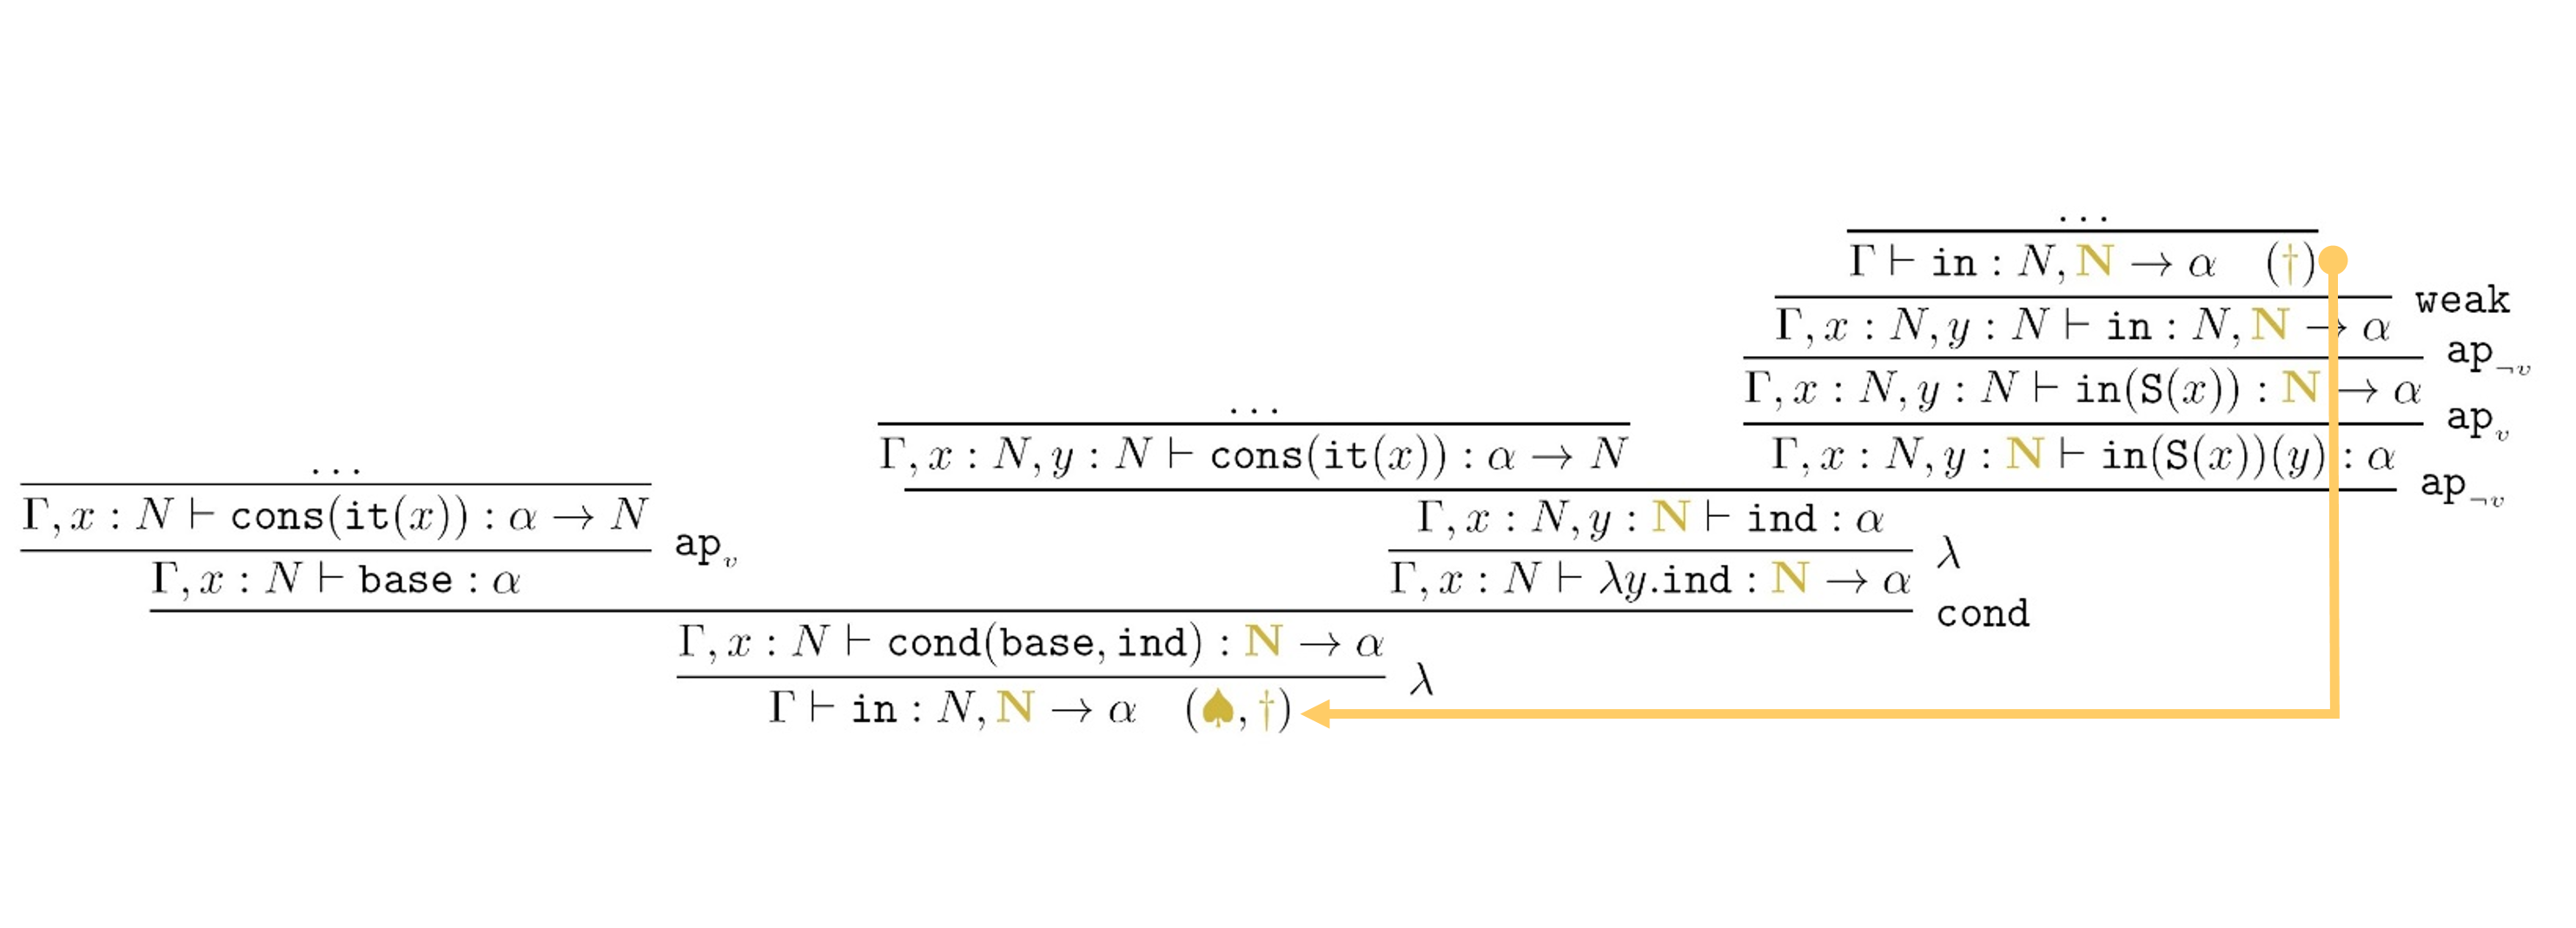
\includegraphics[scale=0.6]{type-inference-term-interval.PNG}

\begin{center}
%% LATEX SOURCE CODE THEN A SNAPSHOT 
%% THEN THE SNAPSHOT HAS BEEN MODIFIED IN WORD 
%% THEN A LAST SNAPSHOT
  
\[
%\infer[\lambda]
% {\Sigma\vdash \Interval:(\N \rightarrow \N),\N,\N,\bfColor{oldgold}{\N}\rightarrow\alpha}
% {\infer[\lambda]
%   {\Sigma,f:\N\rightarrow\N \vdash \lambda a.\interval:\N,\N,\bfColor{oldgold}{\N}   
%      \rightarrow\alpha}
   {\infer[\lambda]  
     {\Gamma \vdash \interval:\N,\bfColor{oldgold}{\N}\rightarrow\alpha 
       \ \ \ (\bfColor{oldgold}{\dagger}) }
       {\infer[\cond]{\Gamma, x:\N 
	\vdash 
	\cond (\base,  \inductive )
	:\bfColor{oldgold}{\N}\rightarrow\alpha \ \ \ (\bfColor{oldgold}{ \spadesuit}) } 
       {\infer[\apvar]{\Gamma, x:\N 
	           \vdash 
	           \base:\alpha}
             {\infer[]{\Gamma, x:\N 
	           \vdash 
	           \cons(\iter(x)):\alpha \rightarrow\N}{\ldots}}
            {\ \ \ \ \ \ }  &
          \infer[\lambda]{\Gamma, x:\N 
	           \vdash 
	           \lambda y.\inductive : \bfColor{oldgold}{\N}\rightarrow\alpha}
             {\infer[\apnotvar]{\Gamma, x:\N, y:\bfColor{oldgold}{\N} \vdash
               \inductive : \alpha}
            {\infer[]
                     {\Gamma, x:\N, y:\N 
                          \vdash \cons(\iter(x)):\alpha\rightarrow\N}{\ldots}
               {\ \ \ \ \ \ }
                     {\infer[\apvar]{\Gamma, x:\N, y:\bfColor{oldgold}{\N} 
                          \vdash \interval(\Succ(x))(y):\alpha}
                         {\infer[\apnotvar]{\Gamma, x:\N, y:\N 
                          \vdash \interval(\Succ(x)):\bfColor{oldgold}{\N} \rightarrow\alpha}
                              {\infer[\weak]{\Gamma, x:\N, y:\N 
                          \vdash \interval:\N,\bfColor{oldgold}{\N} \rightarrow\alpha}
                                {\infer[]{\Gamma 
                          \vdash \interval:\N,\bfColor{oldgold}{\N} \rightarrow\alpha
                           \ \ \ (\bfColor{oldgold}{\dagger})}
              {\ldots}}}}}
             }
           }
         }
       }  
    }
%   }
\]

\mbox{Figure \ref{figure-term-interval}}
\end{center}

\end{figure}

If we carefully examine the term $\Interval$, we can guess several results of this paper.
We have infinitely many nested $\beta$-reduction $(\lambda x. \ldots)(\Succ (x))$.
We can remove all of them in a single step. Inside the $\beta$-redex number $k$ we obtain a sub-term
$\iter[\Succ (x)/x]\ldots[\Succ (x)/x]$ (substitution repeated $k$ times).
The result is $\iter[\Succ ^k(x)/x] $.
The nested substitution produce infinitely many pairwise different sub-terms 
$\iter(\Succ ^k(x))$ for all $k \in \N$.
We need infinitely many steps to normalize all $\iter(\Succ ^k(x))$ to $f^k(I)$, 
even if we allow to reduce all $\beta,\cond$-redexes at the same time.
Also the normal form is not regular: it contains all terms $f^k(\iter(x))$ for $k \in \N$, hence
infinitely many pairwise different terms. 
%These infinite sub-terms are of a particulary simple form, though. 
%They are obtained by the repeating $k$ times the assignment $z:=f(z)$, then applying $z:=I$ once
%to the result.

In conclusion, 
$\Interval$ is some term of $\CTlambda$ which can be safely normalized, but which 
cannot be fully normalized in finite time, not even if we allow
infinite parallel reductions without any "safety" restriction. 
The normal form is produced \emph{only in the limit}
and it is \emph{not regular}. If we allow to reduce infinitely many nested existing
$\beta$-redexes in one step, also
the intermediate steps of the infinite reduction of $\Interval$ are not regular.


%16:32 30/04/2024
%22:30 03/06/2024

